\subsection{Diagrams}
All planar/string diagrams are to be read from bottom to top.

Let $A,C,D,E$ be $\CC$-vector spaces.
\begin{itemize}
 \item
  The identity on $A$ is given by the string $\begin{tikzpicture}[rotate=90, xshift=-0.5cm,
   baseline=-\dimexpr\fontdimen22\textfont2\relax]
    \draw (0,0)--(1,0);
    \path (-0.25,0) node[font=\normalsize] {$A$};
    \path (1.25,0) node[font=\normalsize] {$A$};
   \end{tikzpicture}$\,.
 \item A linear map $f\colon{A}\to{C}$ is given by the string $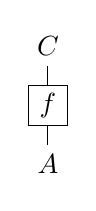
\begin{tikzpicture}[rotate=90,
  xshift=-0.5cm,
  baseline=-\dimexpr\fontdimen22\textfont2\relax]
  \draw (0,0)--(1,0);
  \path[draw,fill=white] (0.25,-0.25) rectangle (0.75,0.25);
  \path (0.5,0) node[font=\normalsize] {$f$};
  \path (-0.25,0) node[font=\normalsize] {$A$};
  \path (1.25,0) node[font=\normalsize] {$C$};
 \end{tikzpicture}$\,.
 \item Inputting an element $x\in{A}$ can be shown by the string
  $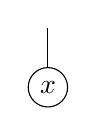
\begin{tikzpicture}[rotate=90,
   xshift=-0.5cm,
   baseline=-\dimexpr\fontdimen22\textfont2\relax]
    \draw (0,0)--(1,0);
    \path[draw,fill=white] (0.25,0) circle[radius=0.25cm];
    \path (0.25,0) node[font=\normalsize] {$x$};
   \end{tikzpicture}$\,.
 \item 
  So then $f(x)$ is shown as
   $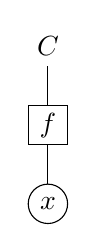
\begin{tikzpicture}[rotate=90,
    xshift=-1.25cm,
    baseline=-\dimexpr\fontdimen22\textfont2\relax]
     \draw (0,0)--(2,0);
     \path[draw, fill=white] (1,-0.25) rectangle (1.5,0.25);
     \path[draw,fill=white] (0.25,0) circle[radius=0.25cm];
     \path (0.25,0) node[font=\normalsize] {$x$};
     \path (1.25,0) node[font=\normalsize] {$f$};
     \path (2.25,0) node[font=\normalsize] {$C$};
    \end{tikzpicture}\,=\,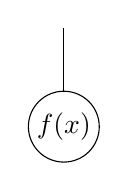
\begin{tikzpicture}[rotate=90,
      xshift=-0.5cm,
      baseline=-\dimexpr\fontdimen22\textfont2\relax]
      \draw (0,0)--(1.5,0);
      \path[draw,fill=white] (0.25,0) circle[radius=0.45cm];
      \path (0.25,0) node[font=\normalsize] {$f(x)$};
     \end{tikzpicture}$\,.
 \item Given $g\colon{D\to{A}}$, we have $f\circ g$ is given by $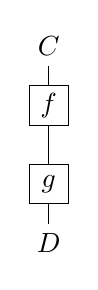
\begin{tikzpicture}[rotate=90,
  xshift=-1cm,
  baseline=-\dimexpr\fontdimen22\textfont2\relax]
  \draw (0,0)--(2,0);
  \path[draw,fill=white] (0.25,-0.25) rectangle (0.75,0.25);
  \path[draw,fill=white] (1.25,-0.25) rectangle (1.75,0.25);
  \path (0.5,0) node[font=\normalsize] {$g$};
  \path (1.5,0) node[font=\normalsize] {$f$};
  \path (-0.25,0) node[font=\normalsize] {$D$};
  \path (2.25,0) node[font=\normalsize] {$C$};
 \end{tikzpicture}$\,.
 \item Given $s\colon{D\to E}$, we have $f\otimes s$ is given by $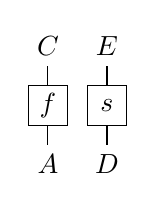
\begin{tikzpicture}[rotate=90,
      xshift=-0.5cm,
      baseline=-\dimexpr\fontdimen22\textfont2\relax]
      \draw (0,0)--(1,0);
      \path[draw,fill=white] (0.25,-0.25) rectangle (0.75,0.25);
      \path (0.5,0) node[font=\normalsize] {$f$};
      \path (-0.25,0) node[font=\normalsize] {$A$};
      \path (1.25,0) node[font=\normalsize] {$C$};
      \begin{scope}[yshift=-0.75cm]
       \draw (0,0)--(1,0);
       \path[draw,fill=white] (0.25,-0.25) rectangle (0.75,0.25);
       \path (0.5,0) node[font=\normalsize] {$s$};
       \path (-0.25,0) node[font=\normalsize] {$D$};
       \path (1.25,0) node[font=\normalsize] {$E$};
      \end{scope}
     \end{tikzpicture}$\,.
 \item Similarly, inputting an element $x\otimes y$ for $x\in{A}$ and $y\in{D}$, is given by
    $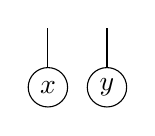
\begin{tikzpicture}[rotate=90,
      xshift=-0.5cm,
      baseline=-\dimexpr\fontdimen22\textfont2\relax]
      \draw (0,0)--(1,0);
      \path[draw,fill=white] (0.25,0) circle[radius=0.25cm];
      \path (0.25,0) node[font=\normalsize] {$x$};
      \begin{scope}[yshift=-0.75cm]
       \draw (0,0)--(1,0);
       \path[draw,fill=white] (0.25,0) circle[radius=0.25cm];
       \path (0.25,0) node[font=\normalsize] {$y$};
      \end{scope}
     \end{tikzpicture}$\,.
 \item Define $\varkappa_{A,D}$ as the identification $A\otimes D\cong D\otimes A$ given by $x\otimes y\mapsto y\otimes x$. The string diagram of $\varkappa_{A,D}$ is given by
   $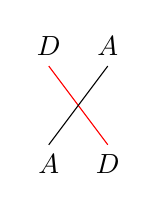
\begin{tikzpicture}[rotate=90,
      xshift=-0.5cm,
      baseline=-\dimexpr\fontdimen22\textfont2\relax]
      \draw[red] (0,0)--(1,0.75);
      \draw (1,0)--(0,0.75);
      \path (-0.25,0) node[font=\normalsize] {$D$};
      \path (-0.25,0.75) node[font=\normalsize] {$A$};
      \path (1.25,0) node[font=\normalsize] {$A$};
      \path (1.25,0.75) node[font=\normalsize] {$D$};
     \end{tikzpicture}
     =
     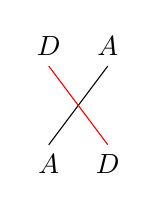
\begin{tikzpicture}[rotate=90,
      xshift=-0.5cm,
      baseline=-\dimexpr\fontdimen22\textfont2\relax]
      \draw (1,0)--(0,0.75);
      \draw[red] (0,0)--(1,0.75);
      \path (-0.25,0) node[font=\normalsize] {$D$};
      \path (-0.25,0.75) node[font=\normalsize] {$A$};
      \path (1.25,0) node[font=\normalsize] {$A$};
      \path (1.25,0.75) node[font=\normalsize] {$D$};
     \end{tikzpicture}$\,.\\
    The red and blue strands are meant to highlight the fact that they are not intersecting, but overlapping (either way).\\
    So then it is clear that for any $x\in{D}$ and $y\in{A}$, we get,
    $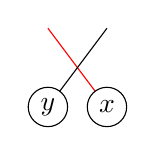
\begin{tikzpicture}[rotate=90,
      xshift=-0.5cm,
      baseline=-\dimexpr\fontdimen22\textfont2\relax]
      \draw[red] (0,0)--(1,0.75);
      \draw (1,0)--(0,0.75);
      \draw[fill=white] (0,0) circle[radius=0.25cm];
      \draw[fill=white] (0,0.75) circle[radius=0.25cm];
      \draw (0,0) node[font=\normalsize] {$x$};
      \draw (0,0.75) node[font=\normalsize] {$y$};
     \end{tikzpicture}
     =
     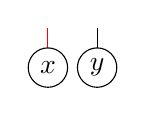
\begin{tikzpicture}[rotate=90,
      xshift=-0.5cm,
      baseline=-\dimexpr\fontdimen22\textfont2\relax]
      \draw[red] (0.5,0.375)--(1,0.375);
      \draw (0.5,-0.25)--(1,-0.25);
      \draw[fill=white] (0.5,-0.25) circle[radius=0.25cm];
      \draw[fill=white] (0.5,0.375) circle[radius=0.25cm];
      \draw (0.5,0.375) node[font=\normalsize] {$x$};
      \draw (0.5,-0.25) node[font=\normalsize] {$y$};
     \end{tikzpicture}$.
 \item When $A$ and $C$ are Hilbert spaces, then the adjoint of $f\in\Bcal(A,C)$ is given by the string diagram $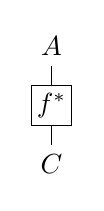
\begin{tikzpicture}[rotate=90, xshift=-0.5cm,
   baseline=-\dimexpr\fontdimen22\textfont2\relax]
    \draw (0,0)--(1,0);
    \path[draw,fill=white] (0.25,-0.25) rectangle (0.75,0.25);
    \path (0.5,0) node[font=\normalsize] {$f^*$};
    \path (-0.25,0) node[font=\normalsize] {$C$};
    \path (1.25,0) node[font=\normalsize] {$A$};
   \end{tikzpicture}$\,,
  in other words, the string diagram of the adjoint of $f$ is given by vertically reflecting the diagram of $f$.
\end{itemize}

Deforming, i.e., stretching, compressing, and/or moving around the strings, retains equality of the diagrams. So we can perform planar isotopies (RO), Reidemeister moves (RII), and Reidemeister moves (RIII).
In knot theory, (RII) and (RIII) moves are shown as follows,
\begin{center}
 \begin{figure}[H]
    \centering
    \begin{minipage}{0.3\textwidth}
    \begin{center}
        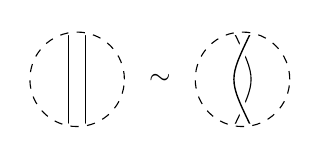
\begin{tikzpicture}[scale=0.3]
            \begin{scope}
            \draw[black] (100:2) -- (260:2);
            \draw[black] ( 80:2) -- (280:2);
            \draw[white,ultra thick] (0,0) circle(2);
            \draw[black,dashed] (0,0) circle(2);
            \end{scope}
            \begin{scope}[xshift=7cm]
            \node[black,scale=1] at (-3.5,0) {$\sim$};
            \draw[black] (100:2) .. controls ( 0.6,0) .. (260:2); 
            \draw[draw=white,double=black,ultra thick,,double distance=0.5pt] ( 80:2) .. controls (-0.6,0) .. (280:2);
            \draw[white,ultra thick] (0,0) circle(2);
            \draw[black,dashed] (0,0) circle(2);
            \end{scope}
        \end{tikzpicture}
    \par{(RII)}
    \end{center}
    \end{minipage}%
    \begin{minipage}{0.3\textwidth}
        \begin{center}
        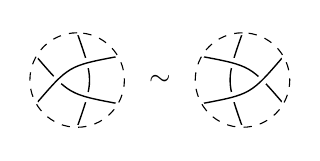
\begin{tikzpicture}[scale=0.3]
        \begin{scope}[rotate=90]
        \draw[draw=white,double=black ,ultra thick,double distance=0.5pt] (  0:2) .. controls (270:0.7) .. (180:2);
        \draw[draw=white,double=black  ,ultra thick,double distance=0.5pt] ( 60:2) .. controls (150:0.7) .. (240:2);
        \draw[draw=white,double=black,ultra thick,double distance=0.5pt] (120:2) .. controls ( 30:0.7) .. (300:2);
        \draw[white,ultra thick] (0,0) circle(2);
        \draw[black,dashed] (0,0) circle(2);
        \end{scope}
        \begin{scope}[xshift=7cm]
        \node[black,scale=1] at (-3.5,0) {$\sim$};
        \end{scope}
        \begin{scope}[xshift=7cm, rotate=90]
        \draw[draw=white,double=black ,ultra thick,double distance=0.5pt] (  0:2) .. controls ( 90:0.7) .. (180:2);
        \draw[draw=white,double=black  ,ultra thick,double distance=0.5pt] ( 60:2) .. controls (330:0.7) .. (240:2);
        \draw[draw=white,double=black,ultra thick,double distance=0.5pt] (120:2) .. controls (210:0.7) .. (300:2);
        \draw[white,ultra thick] (0,0) circle(2);
        \draw[black,dashed] (0,0) circle(2);
        \end{scope}
        \end{tikzpicture}
    \par{(RIII)}
    \end{center}
    \end{minipage}
 \end{figure}
\end{center}
For our string diagrams, we alter the above definition of (RII) and (RIII) moves so that there are no over and under crossings.

It is easy to see that string diagrams retain invariance under regular isotopy.
In particular, (RII) moves on string diagrams can be seen by the following,
\[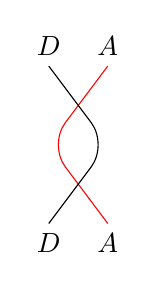
\begin{tikzpicture}[rotate=90,
      xshift=-1cm,
      baseline=-\dimexpr\fontdimen22\textfont2\relax]
      \draw[rounded corners=0.35cm, red] (0,0)--(1,0.75)--(2,0);
      \draw[rounded corners=0.35cm] (2,0.75) -- (1,0)--(0,0.75);
      \path (-0.25,0) node[font=\normalsize] {$A$};
      \path (-0.25,0.75) node[font=\normalsize] {$D$};
      \path (2.25,0) node[font=\normalsize] {$A$};
      \path (2.25,0.75) node[font=\normalsize] {$D$};
     \end{tikzpicture}\simeq\begin{tikzpicture}[rotate=90,
      xshift=-1cm,
      baseline=-\dimexpr\fontdimen22\textfont2\relax]
      \draw[red] (0,0)--(2,0);
      \draw (0,0.75)--(2,0.75);
      \path (-0.25,0) node[font=\normalsize] {$A$};
      \path (-0.25,0.75) node[font=\normalsize] {$D$};
      \path (2.25,0) node[font=\normalsize] {$A$};
      \path (2.25,0.75) node[font=\normalsize] {$D$};
     \end{tikzpicture}\]
The diagram at the left-hand side is exactly $\varkappa_{D,A}\varkappa_{A,D}$, which is the identity, which is exactly what the diagram at the right-hand side represents. This means $\varkappa_{A,D}^*=\varkappa^{-1}_{A,D}$:
\begin{proposition}\label{tensor_product.comm_adjoint}
 $\varkappa_{A,D}^*=\varkappa^{-1}_{A,D}=\varkappa_{D,A}$.
 In other words,
 \[{\left(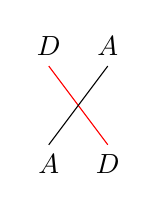
\begin{tikzpicture}[rotate=90,
      xshift=-0.5cm,
      baseline=-\dimexpr\fontdimen22\textfont2\relax]
      \draw[red] (0,0)--(1,0.75);
      \draw (1,0)--(0,0.75);
      \path (-0.25,0) node[font=\normalsize] {$D$};
      \path (-0.25,0.75) node[font=\normalsize] {$A$};
      \path (1.25,0) node[font=\normalsize] {$A$};
      \path (1.25,0.75) node[font=\normalsize] {$D$};
     \end{tikzpicture}\right)}^*=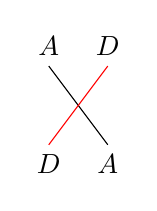
\begin{tikzpicture}[rotate=90,
      xshift=-0.5cm,
      baseline=-\dimexpr\fontdimen22\textfont2\relax]
      \draw (0,0)--(1,0.75);
      \draw[red] (1,0)--(0,0.75);
      \path (-0.25,0) node[font=\normalsize] {$A$};
      \path (-0.25,0.75) node[font=\normalsize] {$D$};
      \path (1.25,0) node[font=\normalsize] {$D$};
      \path (1.25,0.75) node[font=\normalsize] {$A$};
     \end{tikzpicture}\,.\]\qed
\end{proposition}
\begin{proof}
 Let $x,w\in A$ and $y,z\in D$. Then we compute,
 \begin{align*}
  \ip{x\otimes{y}}{\varkappa_{A,D}^*(z\otimes{w})}_{A\otimes D} &= \ip{y\otimes{x}}{z\otimes{w}}_{D \otimes A}
  = \ip{y}{z}_{A}\ip{x}{w}_{D}\\
  &= \ip{x\otimes{y}}{w\otimes{z}}_{A \otimes D}
  = \ip{x\otimes{y}}{\varkappa_{A,D}^{-1}(z\otimes{w})}_{A\otimes D}.
 \end{align*}
 Thus $\varkappa_{A,D}^*=\varkappa_{A,D}^{-1}$.
\end{proof}

Similarly, (RIII) can be seen by the following,
\[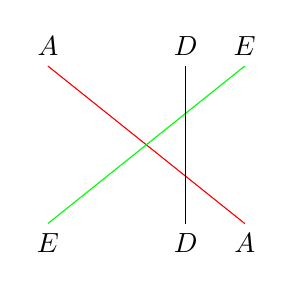
\begin{tikzpicture}[rotate=90,
      xshift=-1cm,
      baseline=-\dimexpr\fontdimen22\textfont2\relax]
      \draw[red] (0,0)--(2,2.5);
      \draw[green] (0,2.5)--(2,0);
      \draw (0,0.75)--(2,0.75);
      \path (-0.25,0) node[font=\normalsize] {$A$};
      \path (-0.25,0.75) node[font=\normalsize] {$D$};
      \path (-0.25,2.5) node[font=\normalsize] {$E$};
      \path (2.25,0) node[font=\normalsize] {$E$};
      \path (2.25,0.75) node[font=\normalsize] {$D$};
      \path (2.25,2.5) node[font=\normalsize] {$A$};
     \end{tikzpicture}\simeq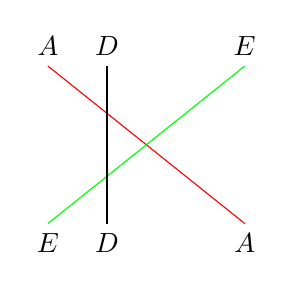
\begin{tikzpicture}[rotate=90,
      xshift=-1cm,
      baseline=-\dimexpr\fontdimen22\textfont2\relax]
      \draw[red] (0,0)--(2,2.5);
      \draw[green] (0,2.5)--(2,0);
      \draw (0,1.75)--(2,1.75);
      \path (-0.25,0) node[font=\normalsize] {$A$};
      \path (-0.25,1.75) node[font=\normalsize] {$D$};
      \path (-0.25,2.5) node[font=\normalsize] {$E$};
      \path (2.25,0) node[font=\normalsize] {$E$};
      \path (2.25,1.75) node[font=\normalsize] {$D$};
      \path (2.25,2.5) node[font=\normalsize] {$A$};
     \end{tikzpicture}\]
The diagram at the left-hand side is exactly $(\id\otimes\,\varkappa_{E,D})(\varkappa_{E,A}\otimes\id)(\id\otimes\,\varkappa_{D,A})$, and the diagram at the right-hand side is exactly $(\varkappa_{D,A}\otimes\id)(\id\otimes\,\varkappa_{E,A})(\varkappa_{E,D}\otimes\id)$. An easy and quick computation shows that these two equations are equal (they both flip the first and last tensor-element and keep the second in place).

\begin{lemma}\label{tensor_product.comm_map}
 Given linear maps $T\colon A\to{D}$ and $S\colon E\to{F}$, we get
 \[\varkappa_{D,F}(T \otimes S)=(S\otimes T)\varkappa_{A,E}.\]
 In other words,
 \[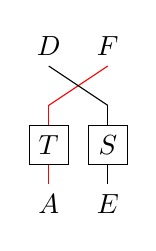
\begin{tikzpicture}[rotate=90,
      xshift=-0.5cm,
      baseline=-\dimexpr\fontdimen22\textfont2\relax]
      \draw[red] (0,0)--(1,0);
      \path[draw,fill=white] (0.25,-0.25) rectangle (0.75,0.25);
      \path (0.5,0) node[font=\normalsize] {$T$};
      \path (-0.25,0) node[font=\normalsize] {$A$};
      \path (1.75,0) node[font=\normalsize] {$D$};
      \draw (0,-0.75)--(1,-0.75);
      \draw[red] (1,0) -- (1.5,-0.75);
      \draw (1,-0.75) -- (1.5,0);
      \path[draw,fill=white] (0.25,-1) rectangle (0.75,-0.5);
      \path (0.5,-0.75) node[font=\normalsize] {$S$};
      \path (-0.25,-0.75) node[font=\normalsize] {$E$};
      \path (1.75,-0.75) node[font=\normalsize] {$F$};
     \end{tikzpicture}
   =
    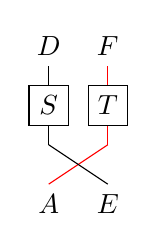
\begin{tikzpicture}[rotate=-90,
      xshift=-1cm,
      % xscale=-1,
      baseline=-\dimexpr\fontdimen22\textfont2\relax]
      \draw[red] (0,0)--(1,0);
      \path[draw,fill=white] (0.25,-0.25) rectangle (0.75,0.25);
      \path (0.5,0) node[font=\normalsize] {$T$};
      \path (-0.25,0) node[font=\normalsize] {$F$};
      \path (1.75,0) node[font=\normalsize] {$E$};
      \draw (0,-0.75)--(1,-0.75);
      \draw[red] (1,0) -- (1.5,-0.75);
      \draw (1,-0.75) -- (1.5,0);
      \path[draw,fill=white] (0.25,-1) rectangle (0.75,-0.5);
      \path (0.5,-0.75) node[font=\normalsize] {$S$};
      \path (-0.25,-0.75) node[font=\normalsize] {$D$};
      \path (1.75,-0.75) node[font=\normalsize] {$A$};
     \end{tikzpicture}\]\qed
\end{lemma}
\begin{proof}
 Let $x\in{A}$ and $y\in{E}$. Then,
 \[\varkappa_{D,F}(T\otimes S)(x\otimes y)=\varkappa_{D,F}(T(x)\otimes S(y))=S(y)\otimes T(x)=(S\otimes T)\varkappa_{A,E}(x\otimes y).\]
 Pictorially, one can see this by simply sliding the linear maps across the strand to the other side of the crossing.
\end{proof}
